\chapter{Drawing conclusions}
\label{ch:grand-finale}

\section{The main equivalence}
In general, we can define a monoidal functor by just evaluating it on the generators of the source category.
In our case, where a two-dimensional TQFT is a symmetric monoidal functor $Z \colon \bord{2} \to \mathbf{Vect}_\Bbbk$, this implies that $Z$ is entirely described by its evaluation on the generating morphisms (and the objects of the skeleton).

Following the definition of a TQFT we then choose a $\Bbbk$-vector space $A$ as the image of the circle 
\[
(\mathbf{1}) \mapsto A
\] 
and, by functoriality, 
\[
\bordcylinder \mapsto [\id_A \colon A \to A]
\] 
Being $Z$ a symmetric monoidal functor, it also follows that
\[
(\mathbf{n}) \mapsto A \tensor \dots \tensor A = A^{\tensor n}
\hspace{3em}\text{and}\hspace{3em}
\bordtwist \mapsto [\sigma\colon A \tensor A \to A \tensor A]
\]
The images of the remaining generators are defined as follows
\begin{align*}
    \bordcap & \mapsto [\eta \colon \Bbbk \to A] \hspace{3.5em} \wireunit \\
    \bordpants  & \mapsto [\mu \colon A \tensor A \to A] \hspace{1em} \wiremult \\
    \bordcocap  & \mapsto [\varepsilon \colon A \to \Bbbk] \hspace{3.5em} \wirecounit \\
    \bordcopants  & \mapsto [\delta \colon A \to A \tensor A] \hspace{1em} \wirecomult
\end{align*}
The relations in $\bord{2}$ then become relations between these $\Bbbk$-linear maps. For example, for the handle cancellation, we have:
\[
\begin{tikzpicture}[every tqft/.style={transform shape, bottom color=gray, top color=white, fill opacity=0.5}, tqft/view from=incoming, tqft/boundary separation=1.5cm, rotate=-90, scale=0.4, baseline=-2pt]
    \pic[tqft pair of pants, name=a, draw,
    every incoming lower boundary component/.style={draw}, 
    anchor=incoming boundary 1, 
    every incoming boundary component/.style={fill=gray, fill opacity=0.7}];
    \pic[tqft cup, anchor=incoming boundary 1, name=b, at=(a-outgoing boundary 1), draw, every lower boundary component/.style={dashed, draw}];
    \pic[tqft cylinder, anchor=incoming boundary 1, name=c, at=(a-outgoing boundary 2), draw, every lower boundary component/.style={dashed, draw}];
\end{tikzpicture}
= 
\begin{tikzpicture}[every tqft/.style={transform shape, bottom color=gray, top color=white, fill opacity=0.5}, tqft/view from=incoming, tqft/boundary separation=1.5cm, rotate=-90, scale=0.4, baseline=-2pt]
    \pic[tqft cylinder, name=a, draw, every incoming lower boundary component/.style={draw}, every outgoing lower boundary component/.style={dashed, draw}, anchor=outgoing boundary 1, every incoming boundary component/.style={fill=gray, fill opacity=0.7}];
\end{tikzpicture}
=
\begin{tikzpicture}[every tqft/.style={transform shape, bottom color=gray, top color=white, fill opacity=0.5}, tqft/view from=incoming, tqft/boundary separation=1.5cm, rotate=-90, scale=0.4, baseline=-2pt]
    \pic[tqft pair of pants, name=a, draw, every incoming lower boundary component/.style={draw}, anchor=incoming boundary 1, every incoming boundary component/.style={fill=gray, fill opacity=0.7}];
    \pic[tqft cup, anchor=incoming boundary 1, name=b, at=(a-outgoing boundary 2), draw, every lower boundary component/.style={dashed, draw}];
    \pic[tqft cylinder, anchor=incoming boundary 1, name=c, at=(a-outgoing boundary 1), draw, every lower boundary component/.style={dashed, draw}];
\end{tikzpicture}
\hspace{1em}\text{becomes}\hspace{1em}
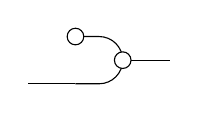
\begin{tikzpicture}[x=0.6cm, y=0.3cm, baseline]
    \draw[rounded corners=0.3cm] (-1,1) -- (0,1) -- (0,0);
    \draw[rounded corners=0.3cm] (-1,-1) -- (0,-1) -- (0,0);
    \draw (-1,-1) -- (-2,-1);
    \draw (0,0) -- (1,0);
    \draw[fill=white] (0,0) circle (3pt);
    \draw[fill=white] (-1,1) circle (3pt);
\end{tikzpicture}
\:=\:
\begin{tikzpicture}[x=0.6cm, y=0.3cm, baseline]
    \draw (0,0) -- (1,0);    
\end{tikzpicture}
\:=\:
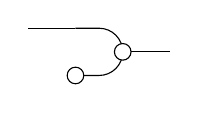
\begin{tikzpicture}[x=0.6cm, y=0.3cm, baseline]
    \draw[rounded corners=0.3cm] (-1,1) -- (0,1) -- (0,0);
    \draw[rounded corners=0.3cm] (-1,-1) -- (0,-1) -- (0,0);
    \draw (-1,1) -- (-2,1);
    \draw (0,0) -- (1,0);
    \draw[fill=white] (0,0) circle (3pt);
    \draw[fill=white] (-1,-1) circle (3pt);
\end{tikzpicture}
\]

By ``slimming'' all the relations in $\bord{2}$, it should becomes obvious there exists some kind of relation between topological quantum field theories and the Frobenius structure we studied in the previous chapter. 
These considerations lead us to the main theorem regarding the classification of 2-dimensional TQFTs.
\begin{tcbthm}
    There is a canonical equivalence of categories between 2-dimensional TQFTs taking values in $\mathbf{Vect}_\Bbbk$ and commutative Frobenius $\Bbbk$-algebras.
    \[
    \mathbf{2TQFT}_\Bbbk \iso \mathbf{cFA}_\Bbbk
    \]
\end{tcbthm}

Thanks to our journey through the previous chapters the proof becomes straightforward. We can now explicitly bulid the correspondence, for both objects and arrows.

Indeed, given an object $Z$ in $\textbf{2TQFT}_\Bbbk$ we get the axioms defining a structure of commutative Frobenius algebra on the vector space $Z((\mathbf{1})) = A$.

\[
\begin{tikzpicture}[every tqft/.style={transform shape, bottom color=gray, top color=white, fill opacity=.5}, tqft/view from=incoming, tqft/boundary separation=1.5cm, rotate=-90, scale=0.4, baseline=-2pt]
    \pic[tqft reverse pair of pants, name=a, draw, every lower boundary component/.style={dashed, draw}, anchor=outgoing boundary 1];
    \pic[tqft cap, anchor=outgoing boundary 1, name=b, at=(a-incoming boundary 1), draw];
    \pic[tqft cylinder, anchor=outgoing boundary 1, name=c, at=(a-incoming boundary 2), draw, every incoming lower boundary component/.style={draw}, every incoming boundary component/.style={fill=gray, fill opacity=0.7}];
\end{tikzpicture}
= 
\begin{tikzpicture}[every tqft/.style={transform shape, bottom color=gray, top color=white, fill opacity=0.5}, tqft/view from=incoming, tqft/boundary separation=1.5cm, rotate=-90, scale=0.4, baseline=-2pt]
    \pic[tqft cylinder, name=a, draw, every incoming lower boundary component/.style={draw}, every outgoing lower boundary component/.style={dashed, draw}, anchor=incoming boundary 1, every incoming boundary component/.style={fill=gray, fill opacity=0.7}];
\end{tikzpicture}
=
\begin{tikzpicture}[every tqft/.style={transform shape, bottom color=gray, top color=white, fill opacity=.5}, tqft/view from=incoming, tqft/boundary separation=1.5cm, rotate=-90, scale=0.4, baseline=-2pt]
    \pic[tqft reverse pair of pants, name=a, draw, every lower boundary component/.style={dashed, draw}, anchor=outgoing boundary 1];
    \pic[tqft cap, anchor=outgoing boundary 1, name=b, at=(a-incoming boundary 2), draw];
    \pic[tqft cylinder, anchor=outgoing boundary 1, name=c, at=(a-incoming boundary 1), draw, every incoming lower boundary component/.style={draw}, every incoming boundary component/.style={fill=gray, fill opacity=0.7}];
\end{tikzpicture}
\hspace{1em}\text{becomes}\hspace{1em}
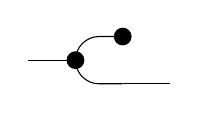
\begin{tikzpicture}[x=0.6cm, y=0.3cm, baseline]
    \draw[rounded corners=0.3cm] (1,1) -- (0,1) -- (0,0);
    \draw[rounded corners=0.3cm] (1,-1) -- (0,-1) -- (0,0);
    \draw (1,-1) -- (2,-1);
    \draw (0,0) -- (-1,0);
    \draw[fill=black] (0,0) circle (3pt);
    \draw[fill=black] (1,1) circle (3pt);
\end{tikzpicture}
\:=\:
\begin{tikzpicture}[x=0.6cm, y=0.3cm, baseline]
    \draw (0,0) -- (1,0);    
\end{tikzpicture}
\:=\:
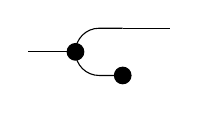
\begin{tikzpicture}[x=0.6cm, y=0.3cm, baseline]
    \draw[rounded corners=0.3cm] (1,1) -- (0,1) -- (0,0);
    \draw[rounded corners=0.3cm] (1,-1) -- (0,-1) -- (0,0);
    \draw (1,1) -- (2,1);
    \draw (0,0) -- (-1,0);
    \draw[fill=black] (0,0) circle (3pt);
    \draw[fill=black] (1,-1) circle (3pt);
\end{tikzpicture}
\]  

\[
\begin{tikzpicture}[every tqft/.style={transform shape, bottom color=gray, top color=white, fill opacity=0.5}, tqft/view from=incoming, tqft/boundary separation=1.5cm, rotate=-90, scale=0.4, baseline=-2pt]
    \pic[tqft pair of pants, name=a, draw, anchor=outgoing boundary 1,
    every incoming lower boundary component/.style={draw}, 
    every incoming boundary component/.style={fill=gray, fill opacity=0.7}];
    \pic[tqft reverse pair of pants, name=b, draw, anchor=incoming boundary 2, at=(a-outgoing boundary 1),
    every lower boundary component/.style={dashed, draw}]; 
    \pic[tqft cylinder to prior, draw, anchor=incoming boundary, at=(a-outgoing boundary 2),
    every lower boundary component/.style={dashed, draw}]; 
    \pic[tqft cylinder to prior, draw, anchor=outgoing boundary, at=(b-incoming boundary 1),
    every incoming lower boundary component/.style={draw}, 
    every incoming boundary component/.style={fill=gray, fill opacity=0.7}]; 
\end{tikzpicture}
=
\begin{tikzpicture}[every tqft/.style={transform shape, bottom color=gray, top color=white, fill opacity=0.5}, tqft/view from=incoming, tqft/boundary separation=1.5cm, rotate=-90, scale=0.4, baseline=-2pt]
    \pic[tqft pair of pants, name=a, draw, 
    every lower boundary component/.style={dashed, draw}];
    \pic[tqft reverse pair of pants, draw, anchor=outgoing boundary, at=(a-incoming boundary),
    every incoming lower boundary component/.style={draw}, 
    every incoming boundary component/.style={fill=gray, fill opacity=0.7}];
\end{tikzpicture}
=
\begin{tikzpicture}[every tqft/.style={transform shape, bottom color=gray, top color=white, fill opacity=0.5}, tqft/view from=incoming, tqft/boundary separation=1.5cm, rotate=-90, scale=0.4, baseline=-2pt]
    \pic[tqft pair of pants, name=a, draw, anchor=outgoing boundary 2,
    every incoming lower boundary component/.style={draw}, 
    every incoming boundary component/.style={fill=gray, fill opacity=0.7}];
    \pic[tqft reverse pair of pants, name=b, draw, anchor=incoming boundary 1, at=(a-outgoing boundary 2),
    every lower boundary component/.style={dashed, draw}]; 
    \pic[tqft cylinder to next, draw, anchor=incoming boundary, at=(a-outgoing boundary 1),
    every lower boundary component/.style={dashed, draw}]; 
    \pic[tqft cylinder to next, draw, anchor=outgoing boundary, at=(b-incoming boundary 2),
    every incoming lower boundary component/.style={draw}, 
    every incoming boundary component/.style={fill=gray, fill opacity=0.7}]; 
\end{tikzpicture}
\hspace{1em}\text{becomes}\hspace{.5em}
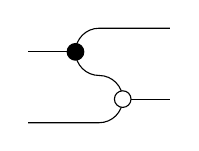
\begin{tikzpicture}[x=0.6cm, y=0.3cm, baseline,yshift=-0.25cm]
    \draw[rounded corners=0.3cm] (0,2) -- (0,1) -- (.5,1);
    \draw[rounded corners=0.3cm] (0,2) -- (0,3) -- (2,3);
    \draw[rounded corners=0.3cm] (1,0) -- (1,1) -- (.5,1);
    \draw[rounded corners=0.3cm] (1,0) -- (1,-1) -- (-1,-1);
    \draw (2,0)--(1,0);
    \draw (0,2)--(-1,2);
    \draw[fill=black] (0,2) circle (3pt);
    \draw[fill=white] (1,0) circle (3pt);
\end{tikzpicture}
\:=\:
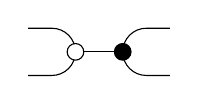
\begin{tikzpicture}[x=0.6cm, y=0.3cm, baseline]
    \draw[rounded corners=0.3cm] (-1,-1) -- (0,-1) -- (0,0);
    \draw[rounded corners=0.3cm] (-1,1) -- (0,1) -- (0,0);
    \draw (0,0) -- (1,0);
    \draw[fill=white] (0,0) circle (3pt);
    \draw[fill=black] (1,0) circle (3pt);
    \draw[rounded corners=0.3cm] (1,0) -- (1,1) -- (2,1);
    \draw[rounded corners=0.3cm] (1,0) -- (1,-1) -- (2,-1);
\end{tikzpicture}
\:=\:
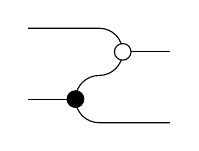
\begin{tikzpicture}[x=0.6cm, y=0.3cm, baseline,yshift=-0.25cm]
    \draw[rounded corners=0.3cm] (0,2) -- (0,1) -- (-.5,1);
    \draw[rounded corners=0.3cm] (0,2) -- (0,3) -- (-2,3);
    \draw[rounded corners=0.3cm] (-1,0) -- (-1,1) -- (-.5,1);
    \draw[rounded corners=0.3cm] (-1,0) -- (-1,-1) -- (1,-1);
    \draw (-2,0)--(-1,0);
    \draw (0,2)--(1,2);
    \draw[fill=white] (0,2) circle (3pt);
    \draw[fill=black] (-1,0) circle (3pt);
\end{tikzpicture}
\]

\[
\begin{tikzpicture}[every tqft/.style={transform shape, bottom color=gray, top color=white, fill opacity=0.5}, tqft/view from=incoming, rotate=-90, scale=0.4, baseline=-2pt]
    \pic[tqft pair of pants, draw, name=a,     
    boundary separation=1.5cm,
    every incoming lower boundary component/.style={draw}, 
    every incoming boundary component/.style={fill=gray, fill opacity=0.7}];   
    \pic[tqft,
    incoming boundary components=1,
    outgoing boundary components=1,
    offset=-.75,
    anchor=incoming boundary,
    at=(a-outgoing boundary 2),
    draw,
    every lower boundary component/.style={dashed, draw}];
    \pic[tqft,
    incoming boundary components=1,
    outgoing boundary components=1,
    offset=.75,
    anchor=incoming boundary,
    at=(a-outgoing boundary 1),
    draw,
    every lower boundary component/.style={dashed, draw}];
\end{tikzpicture}
=
\begin{tikzpicture}[every tqft/.style={transform shape, bottom color=gray, top color=white, fill opacity=0.5}, tqft/view from=incoming, rotate=-90, scale=0.4, baseline=-2pt]
    \pic[tqft pair of pants, draw, name=a,     
    boundary separation=1.5cm,
    every incoming lower boundary component/.style={draw}, 
    every incoming boundary component/.style={fill=gray, fill opacity=0.7},
    every outgoing lower boundary component/.style={dashed, draw}]; 
\end{tikzpicture}
\hspace{1em}\text{becomes}\hspace{1em}
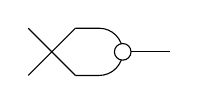
\begin{tikzpicture}[x=0.6cm, y=0.3cm, baseline]
    \draw[rounded corners=0.3cm] (-1,1) -- (0,1) -- (0,0);
    \draw[rounded corners=0.3cm] (-1,-1) -- (0,-1) -- (0,0);
    \draw (0,0) -- (1,0);
    \draw (-2,-1) -- (-1,1);
    \draw (-2,1) -- (-1,-1);
    \draw[fill=white] (0,0) circle (3pt);
\end{tikzpicture}
\:=\:
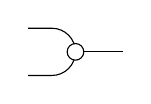
\begin{tikzpicture}[x=0.6cm, y=0.3cm, baseline]
    \draw[rounded corners=0.3cm] (-1,1) -- (0,1) -- (0,0);
    \draw[rounded corners=0.3cm] (-1,-1) -- (0,-1) -- (0,0);
    \draw (0,0) -- (1,0);
    \draw[fill=white] (0,0) circle (3pt);
\end{tikzpicture}
\]
\[
\begin{tikzpicture}[every tqft/.style={transform shape, bottom color=gray, top color=white, fill opacity=0.5}, tqft/view from=incoming, rotate=-90, scale=0.4, baseline=-2pt]
    \pic[tqft reverse pair of pants, anchor=outgoing boundary, draw, name=a,     
    boundary separation=1.5cm,
    every lower boundary component/.style={dashed, draw}];
    \pic[tqft,
    incoming boundary components=1,
    outgoing boundary components=1,
    offset=-.75,
    anchor=outgoing boundary,
    at=(a-incoming boundary 1),
    draw,
    every incoming lower boundary component/.style={draw}, 
    every incoming boundary component/.style={fill=gray, fill opacity=0.7},
    every outgoing lower boundary component/.style={dashed, draw}];
    \pic[tqft,
    incoming boundary components=1,
    outgoing boundary components=1,
    offset=.75,
    anchor=outgoing boundary,
    at=(a-incoming boundary 2),
    draw,
    every incoming lower boundary component/.style={draw}, 
    every incoming boundary component/.style={fill=gray, fill opacity=0.7},
    every outgoing lower boundary component/.style={dashed, draw}];
\end{tikzpicture}
=
\begin{tikzpicture}[every tqft/.style={transform shape, bottom color=gray, top color=white, fill opacity=0.5}, tqft/view from=incoming, rotate=-90, scale=0.4, baseline=-2pt]
    \pic[tqft reverse pair of pants, anchor=outgoing boundary, draw, name=a,     
    boundary separation=1.5cm,
    every incoming lower boundary component/.style={draw}, 
    every incoming boundary component/.style={fill=gray, fill opacity=0.7},
    every outgoing lower boundary component/.style={dashed, draw}]; 
\end{tikzpicture}
\hspace{1em}\text{becomes}\hspace{1em}
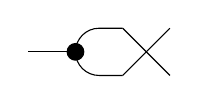
\begin{tikzpicture}[x=0.6cm, y=0.3cm, baseline]
    \draw[rounded corners=0.3cm] (0,0) -- (0,1) -- (1,1);
    \draw[rounded corners=0.3cm] (0,0) -- (0,-1) -- (1,-1);
    \draw (-1,0)--(0,0);
    \draw (1,1)--(2,-1);
    \draw (1,-1)--(2,1);
    \draw[fill=black] (0,0) circle (3pt);
\end{tikzpicture} 
\:=\:
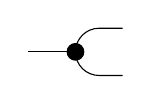
\begin{tikzpicture}[x=0.6cm, y=0.3cm, baseline]
    \draw[rounded corners=0.3cm] (0,0) -- (0,1) -- (1,1);
    \draw[rounded corners=0.3cm] (0,0) -- (0,-1) -- (1,-1);
    \draw (-1,0)--(0,0);
    \draw[fill=black] (0,0) circle (3pt);
\end{tikzpicture} 
\]

Conversely, given a commutative Frobenius algebra $(A, \eta, \mu, \varepsilon, \delta)$, we are able to determine a TQFT by evaluation on the generating morphisms as described above. 

These assignments define a bijection. Starting with a symmetric monoidal functor $Z$ we obtain a commutative Frobenius algebra $A = Z((\mathbf{1}))$. From such algebra we then define a TQFT by mapping $(\mathbf{1})$ onto it, which exactly corresponds to the monoidal functor we started with.

To check this defines an equivalence between the two categories we must also consider what happens to morphisms. By definition, an arrow $u \colon Z \to Z'$ between two 2-dimensional TQFTs is a monoidal natural transformations between the two functors. In particular, the structure of $\bord{2}$, implies that these natural transformations consist of $\Bbbk$-linear maps $A^{\tensor n} \to A'^{\tensor n}$, where $A = Z((\mathbf{1}))$, $A' = Z'((\mathbf{1}))$, compatible with all the arrows in $\bord{2}$. Furthermore, by asking $u$ to be monoidal, these arrows are just the $n$-th tensor power of the $\Bbbk$-linear arrow $u_1 \colon A \to A'$.
Since every arrow in $\bord{2}$ is built by tesoring and gluing the generators, the compatibility of $u$ with the arrows in $\bord{2}$ is entirly determined by the corresponding diagrams. 

\[
\begin{tikzcd}
    \Bbbk \arrow[r, equal] \arrow[d, "\eta"] & \Bbbk \arrow[d, "\eta'"] \\
    A \arrow[r, "u_1"] & A'
\end{tikzcd}
\hspace{3em}
\begin{tikzcd}[column sep=5em]
    A \tensor A \arrow[r, "u_1 \tensor u_1"] \arrow[d, "\mu"] & A' \tensor A' \arrow[d, "\mu'"]\\
    A \arrow[r, "u_1"] & A'
\end{tikzcd}
\]
\[
\begin{tikzcd}
    A \arrow[r, "u_1"] \arrow[d, "\varepsilon"] & A' \arrow[d, "\varepsilon'"] \\
    \Bbbk \arrow[r, equal] & \Bbbk
\end{tikzcd}
\hspace{3em}
\begin{tikzcd}[column sep=5em]
    A \arrow[r, "u_1"] \arrow[d, "\delta"] & A' \arrow[d, "\delta'"] \\
    A \tensor A' \arrow[r, "u_1 \tensor u_1"] & A'\tensor A'
\end{tikzcd}
\]
\[
\begin{tikzcd}[column sep=5em]
    A \tensor A \arrow[r, "u_1 \tensor u_1" ] \arrow[d, "\sigma"] & A' \tensor A' \arrow[d, "\sigma'"] \\
    A \tensor A \arrow[r, "u_1 \tensor u_1"] & A'\tensor A'
\end{tikzcd}
\]

Let us now go back to the definitions of algebra and coalgebra homomorphisms.\todo{add ref} We notice that the commutative diagrams there are formally identical to the naturality condition imposed on the monoidal transformation $u \colon Z \to Z'$. We then have proved that each monoidal transformation in $\bord{2}$ defines a morphism of Frobenius algebras, hence (by symmetry of the functors $Z$ and $Z'$) of commutative ones. 

By applying the same argument backwards we reach the converse implication, thus completing the proof of the categorical equivalence.


\section{A broader result}

\todo[inline]{Let us put everything in the right context...}


\begin{tcbdfn}[Internal monoids]
    \label{dfn:internal-monoid}
    Let $(\cat{C}, \sq, I)$ be a monoidal category. An \emph{internal comonoid} in $\cat{C}$ is an object $M$ equippped with two morphisms
    \[
    \mu \colon M \sq M \to M \quad\text{(multiplication)} 
    \hspace{3em}
    \eta \colon I \to M \quad\text{(unit)}
    \]
    such that the following diagrams commute
    \[
    \begin{tikzcd}
    & M \sq M \sq M \arrow[dr, "\id_M \sq \mu"] \arrow[dl, "\mu \sq \id_M", swap] & \\
    M \sq M \arrow[dr, "\mu", swap] & & M \sq M \arrow[dl, "\mu"] \\
    & M &    
    \end{tikzcd}
    \]
    \[
    \begin{tikzcd}
    & M \sq M \arrow[rd, "\mu"] & & M \sq M \arrow[ld, "\mu", swap]& \\
    I \sq M \arrow[ru, "\eta \sq \id_M"] \arrow[rr, "=", swap]& & M & & M \sq I \arrow[lu, "\id_M \sq \eta", swap] \arrow[ll, "="]  
    \end{tikzcd}
    \]
\end{tcbdfn}

The attentive reader has surely noticed that this definition is given on a strict monoidal category. The reason behind this choice is again \ref{thm:strictification}. The general definition is not so different, we report it below for completeness\footnote{And also because in categories like $(\mathbf{Cat}, \times, \mathbf{1})$, $(\mathbf{Vect}_\Bbbk, \tensor, \Bbbk)$ we do not actually have strict unitality.}.

\begin{dfnx*}[Internal monoids]
    Let $(\cat{C}, \sq, I, \alpha, l, r)$ be a monoidal category. An \emph{internal monoid} in $\cat{C}$ is an object $M$ together with two morphisms
    \[
    \mu \colon M \sq M \to M \quad \text{(multiplication)} 
    \hspace{3em}
    \eta \colon I \to M \quad \text{(unit)}
    \]
    such that the following diagrams commute
    \[
    \begin{tikzcd}[row sep=2em]
    (M \sq M) \sq M \arrow[rr, "\alpha"] \arrow[d, "\mu \sq \id_M"] & & M \sq (M \sq M) \arrow[d, "\id_M \sq \mu"] \\
    M \sq M \arrow[dr, "\mu", swap] & & M \sq M \arrow[dl, "\mu"] \\
    & M &
    \end{tikzcd}
    \]
    \[
    \begin{tikzcd}
    & M \sq M \arrow[rd, "\mu"] & & M \sq M \arrow[ld, "\mu", swap]& \\
    I \sq M \arrow[ru, "\eta \sq \id_M"] \arrow[rr, "l_M", swap]& & M & & M \sq I \arrow[lu, "\id_M \sq \eta", swap] \arrow[ll,"r_M"]  
    \end{tikzcd}
    \]
\end{dfnx*}

By reversing the arrows, we also give the definition of \emph{internal comonoid}. 

\begin{tcbdfn}[Internal comonoids]
    \label{dfn:internal-comonoid}
    Let $(\cat{C}, \sq, I)$ be a monoidal category. An \emph{internal comonoid} in $\cat{C}$ is an object $M$ equippped with two morphisms
    \[
    \delta \colon M \to M \sq M \quad\text{(multiplication)} 
    \hspace{3em}
    \varepsilon \colon M \to I \quad\text{(unit)}
    \]
    such that the following diagrams commute
    \[
    \begin{tikzcd}
    & M \sq M \sq M & \\
    M \sq M \arrow[ur, "\delta \sq \id_M"] & & M \sq M \arrow[ul, "\id_M \sq \delta", swap] \\
    & M \arrow[ul, "\delta"] \arrow[ur, "\delta", swap] &    
    \end{tikzcd}
    \]
    \[
    \begin{tikzcd}
    & M \sq M \arrow[dl, "\varepsilon \sq \id_M", swap] & & M \sq M \arrow[dr, "\id_M \sq \varepsilon"]& \\
    I \sq M & & M \arrow[ul, "\delta", swap] \arrow[ur, "\delta"] \arrow[ll, "="] \arrow[rr, "=", swap] & & M   
    \end{tikzcd}
    \]
\end{tcbdfn}

\todo[inline]{examples: in Set Cat and Vect}

As we did for monoidal categories and $\Bbbk$-algebras we are able to define morphisms between internal monoids and comonoids.

\begin{tcbdfn}[Homomorphisms of internal monoids]
Let $(\cat{C}, \sq, I)$ be a monoidal category. An \emph{homomorphisms of internal monoids} $\varphi \colon (M, \mu, \eta) \to (M', \mu', \eta')$ is a morphism from $M$ to $M'$ such that the following diagrams commute.
\[
\begin{tikzcd}
    M \sq M \arrow[d, "\mu"] \arrow[r, "\varphi"] & M' \sq M' \arrow[d, "\mu'"] \\
    M \arrow[r, "\varphi"] & M'
\end{tikzcd}
\hspace{3em}
\begin{tikzcd}
    M \arrow[rr, "\varphi"] & & M'\\
    & I \arrow[ul, "\eta"] \arrow[ur, "\eta'", swap] &
\end{tikzcd}
\]
\end{tcbdfn}


\begin{tcbdfn}[Homomorphisms of internal comonoids]
Let $(\cat{C}, \sq, I)$ be a monoidal category. An \emph{homomorphisms of internal comonoids} $\phi \colon (M, \delta, \varepsilon) \to (M', \delta', \varepsilon')$ is a morphism from $M$ to $M'$ such that the following diagrams commute.
\[
\begin{tikzcd}
    M \sq M \arrow[r, "\phi"] & M' \sq M' \\
    M \arrow[u, "\delta", swap] \arrow[r, "\phi"] & M' \arrow[u, "\delta'", swap]
\end{tikzcd}
\hspace{3em}
\begin{tikzcd}
    M \arrow[rr, "\phi"] \arrow[dr, "\varepsilon", swap]& & M' \arrow[dl, "\varepsilon'"] \\
    & I &
\end{tikzcd}
\]
\end{tcbdfn}

It is rather easy to check how composition of two morphisms of internal monoids (resp. comonoids) is again a morphism of internal monoids (resp. comonoids). Given a monoidal category $(\cat{C}, \sq, I)$, we can define a new category $\mathbf{Mon}(\cat{C})$ where objects are internal monoids in $\cat{C}$ and arrows are the homomorphisms between them.

\todo[inline]{what are commutative internal monoids??}
\todo[inline]{C symm mon cat implies MonC is monoidal}

We can now construct an equivalence relation in some way analogous to our main one. This will help us generalize it later on.

\begin{tcbdfn}[The simplex category]
    The \emph{simplex category\footnotemark} $\Delta$ is the category defined by taking
    \begin{itemize}
        \item finite totally ordered sets $[n] \coloneq \{ 0, 1, 2, \dots, n-1 \}$ as objects
        \item order preserving maps as arrows
    \end{itemize}
\end{tcbdfn}
\footnotetext{This structure is sometimes referred to as the \emph{skeletal augmented simplex category}.}

We will then have $[0] = \varnothing$, $[1] = \{0\}$, $[2] = \{0, 1\}$ and so on. It is worth noticing that, in the category $\Delta$, $[0]$ is an initial object and $[1]$ is terminal object.


\begin{tcbdfn}[Ordinal sum]
    The \emph{ordinal sum} is a bifunctor $+ \colon \Delta \times \Delta \to \Delta$ defined in the following way.
    \par
    \textbf{(Objects:).} Consider any two objects $[m]$, $[n]$. Their ordinal sum is defined as the object $[m+n]$ with inclusions given by:
    \begin{align*}
        [m] & \to [m+n] & [n] & \to [m+n] \\
        i & \mapsto i & i & \mapsto m + i
    \end{align*}
    \par
    \textbf{(Arrows:)} Consider any two arrows $f \colon [m] \to [n]$, $f' \colon [m'] \to [n']$. Their ordinal sum is $f + f' \colon [m+m'] \to [n+n']$ assigning
    \[
    i \mapsto 
    \begin{cases}
        f(i) & \text{for } i = 0, \dots, m-1 \\
        n + f'(i-m) & \text{for } i = m, \dots, n-1 
    \end{cases}
    \]
\end{tcbdfn}

Internal monoids. ok
Delta category. 
(their relation).


Internal Frobenius objects.
Bord2.
(Their relation).
